%\begin{abstract}
%Skyline is a popular query type which retrieves data objects that are not dominated by any other object with respect to multiple attributes. Skyline queries have broad applications; however, limited studies have been done on skyline in the broadcast data model. No study has been done on flexible skyline query evaluations in this model that can handle a combination of minimum and maximum attributes. In this paper, we propose the depth-first distributed index (DFDI) and the skyline algorithms that incorporate DFDI to efficiently evaluate skyline in broadcast environments. Our extensive simulations show that the proposed algorithms can answer skyline queries in broadcast environments effectively and efficiently.
%\end{abstract}

\section{Introduction}\label{sec-intro}

Skyline is a query type that retrieves data items which are
considered ``interesting objects'' with respect to multiple
attributes of the data set. For example, someone who is planning
for an ocean-view vacation would be interested to find a list of
hotels that are close to the ocean and at the same time not too
expensive. A hypothetical data set of hotels is shown in
Table~\ref{tab:sample_data}(a). The two relevant attributes in
this case are \emph{minimum distance} to the ocean and
\emph{minimum price}. Figure~\ref{fig:skyline} shows the skyline
points in solid dots as the operation finds hotel records that are
successively further from the ocean, but the prices are the best
for such distances. In the figure, hotel $a$ is a skyline point
because it is the closest to the ocean, although it is not the
lowest price. Hotels $b$ and $d$ are part of the skyline because
each have the closest distance at its price. Hotel $k$ is a
skyline point because it is the cheapest of all the hotels.

\begin{figure}[!h]
\centering \subfigure[2-D skyline of hotels of (X = min, Y = min)]{
    
\includegraphics[width=2in]{Figures/skyline_points.eps}
    \label{fig:skyline}
} \subfigure[3-D skyline of stocks with attributes (X = min, Y = min, Z = max)]{
    
\includegraphics[width=2in]{Figures/skyline_points_3d.eps}
    \label{fig:skyline_points_3d}
} \vspace*{-5pt}\caption{Sample skylines.} \vspace*{-5pt}
\end{figure}

\begin{table}[!h]
  \vspace*{-10pt}
  \small
  \centering
  \caption{Sample data sets.}
  \vspace*{5pt}
  \label{tab:sample_data}
  \subfigure[\small 2-D data of Fig 1(a)]{
  \label{tab:sample_data_a}
  \begin{tabular}{|c|c|c|}
  \hline
  {\bf Hotel} & {\bf Dist.} & {\bf Price} \\ \hline\hline
  a & 1 & 8\\
  b & 2 & 6\\
  c & 4 & 7\\
  d & 3.5 & 3\\
  e & 5 & 4\\
  f & 6 & 7.5\\
  g & 7 & 6\\
  h & 7.5 & 8\\
  i & 6.5 & 3\\
  j & 8 & 4\\
  \hline
  \end{tabular}
  }
  \subfigure[\small 3-D data of Fig 1(b)]{
  \label{tab:sample_data_b}
  \begin{tabular}{|c|c|c|c|}
  \hline
  {\bf Co.} & {\bf Price} & {\bf P/E} & {\bf Yield} \\ \hline\hline
  a & 0 & 5 & 2\\
  b & 1 & 4 & 2\\
  c & 1 & 4 & 1\\
  d & 2 & 2 & 0\\
  e & 3 & 0 & 2\\
  f & 3 & 3 & 0\\
  g & 4 & 3 & 0\\
  h & 4 & 2 & 3\\
  i & 7 & 1 & 4\\
  j & 5 & 4 & 0\\
  \hline
  \end{tabular}}
\end{table}


Skyline has broad applications and relevance to many fields.
Skyline computation in realtime streaming systems with frequent
data updates has been studied in~\cite{conf/icde/LinYWL05}
and~\cite{journals/tkde/TaoP06}. For distributed web services,
skyline query solutions have been proposed
in~\cite{conf/edbt/BalkeGZ04}. Skyline query has also been applied
in sensor networks in~\cite{conf/cikm/ChenLY09}. Meanwhile, the
data broadcast model is a scalable way to disseminate data (e.g.,
FM broadcasting). Unlike the on-demand model, such as most of the
services on the Internet, the broadcast model can scale almost
infinitely. However, a challenge and drawback of this model is the
forward-only access characteristic. While many studies have been
done on different query types to support efficient query
evaluation in broadcast
environments~\cite{conf/dexa/HaKCL09,conf/icde/KuZW07,journals/tmc/KuZW08,
journals/vldb/ZhengLLLS09,conf/cikm/Hara02}, to the best of our
knowledge, the work in~\cite{conf/dexa/HaKCL09} is the only study
on skyline query processing in broadcast environments.
Although~\cite{conf/dexa/HaKCL09} considers broadcast efficiency
(more details in Section~\ref{sec:wireless_broadcast}), the
proposed solution is unable to support all possible skyline types
(i.e., combinations of min and max attributes). In addition, the
work did not address details for skyline computation of higher
data dimensions ($>2$ dimensions) as illustrated in
Figure~\ref{fig:skyline_points_3d}, which plots the potential
investment targets (solid dots) based on the stock information in
Table~\ref{tab:sample_data}(b). For each stock listed, we want the
price and price-to-earnings ratio to be minimized and the yield to
be maximized. To address these challenges, we design a flexible
broadcast index and a skyline evaluation algorithm that utilizes
the index to efficiently evaluate skyline queries in broadcast
environments. Specifically, the contributions of this research are
as follows:

\begin{itemize}
\item We design a flexible on-air index that supports skyline
query evaluation in data broadcast environments for an arbitrary
number of data dimensions.

\item We propose an efficient data broadcast skyline query
algorithm which supports users to ask for minimal or maximal
records in each dimension.

\item We evaluate the performance of the proposed algorithms
through extensive experiments.
\end{itemize}

The rest of this paper is organized as follows.
Section~\ref{sec-prelim} provides background knowledge of the
skyline operator and wireless data broadcast.
Section~\ref{sec-related} surveys related works. We introduce our
index structures to facilitate broadcast skyline query in
Section~\ref{sec-index}. In Section~\ref{sec-pruning} we propose
our pruning region based technique for skyline query evaluation.
The experimental validation of our design is presented in
Section~\ref{sec-exp}. We conclude the paper with a discussion of future work in
Section~\ref{bsky-conc}.


\section{Preliminary}\label{sec-prelim}

\subsection{Skyline Query}\label{sec:skyline_operator}

Skyline query is an operation that finds all data records that
are not dominated by any other data records in a given data set. A
record dominates another record if it is as good or better in all
dimensions and better in at least one dimension. Skyline query is
closely related to the maximal vector
problem~\cite{journals/jacm/KungLP75,conf/vldb/GodfreySG05}. Here,
we briefly introduce these concepts.

\begin{definition}[Maximal Vector]\label{def:max_vector}
Given the set of vectors $V$, for $v \in V$, if there does not
exist $u \in V$ such that $u$ $\geq$ $v$ and $u$ $\neq$ $v$, then
$v$ is a maximal vector of $V$.

\begin{equation}\label{eq:max_vector}
    MaxVect(V) = \{v | \forall v, u \in V \mbox{ } \nexists u \geq v\}
\end{equation}

\end{definition}

The comparison operator $\geq$ utilized in
Equation~\ref{eq:max_vector} is defined on vectors such that for
two vectors $u$, $v \in V$, $u$ $\geq$ $v$ if $u_i$ $\geq$ $v_i$
for $i$ = 1 to $n$ and vice versa for the $\leq$ operator. In
other words, a vector $v$ is greater than the other vector $u$ if
and only if all elements of $v$ is \emph{greater than or equal to}
all elements of $u$. The comparison operators for each element of
the vectors are the natural ordering operators defined on each
domain.

The main difference between the maximal vector operation defined
in Definition~\ref{def:max_vector} and the skyline operation is
that the skyline operator defines a set of \emph{preference
specifiers}, $\sigma$, which are to be either \emph{minimal}
(\emph{min}) or \emph{maximal} (\emph{max}) for each dimension.


\begin{definition}[Skyline Operator]\label{def:skyline}
Give a set of tuples, $T$, and a set of preference specifiers,
$\sigma$, the skyline operator is defined as follows:

\begin{equation}\label{eq:skyline}
    Skyline(T, \sigma) = \{t \in T | \nexists s \in T \text{ where } s \succ t \}
\end{equation}

\end{definition}

The dominance relationship $\succ$ in Definition~\ref{def:skyline}
is defined in the following definition.

\begin{definition}[Dominance Relationship]\label{def:dom_rel}
Given two tuples $t_1$ and $t_2$ in $T$, $t_1$ dominates $t_2$ if
and only if all attributes of $t_1$ dominate or equal all
attributes of $t_2$ and at least one attribute of $t_1$ dominates.
Dominance for each attribute depends on the preference specifier,
$\sigma_i$, for that attribute. Given $x$ and $y$ from a certain
domain $D_i$, the dominance for the attributes is defined as
follows:

\begin{enumerate}
\item If $\sigma_i$ = \emph{min}, $x$ dominates $y$ if $x$ $<$
$y$. \item If $\sigma_i$ = \emph{max}, $x$ dominates $y$ if $x$
$>$ $y$.
\end{enumerate}
\end{definition}



%\begin{corollary}\label{co:dom_rel}
%The dominance relationship is transitive, non-reflexive, and
%non-symmetric.
%\end{corollary}

%\begin{proof}
%All three properties can be proven based on the fact that the
%values of each attribute domain are ordered: an attribute $x$ is
%better than $y$ then, $y$ is worse than $x$. The transitive
%property of the dominance relationship follows from
%Definition~\ref{def:dom_rel}, if record $A$ dominates $B$ then all
%attributes of $A$ are equal or better and there is at least one
%attribute that is better; therefore, $B$ dominates $C$ implies
%that all attributes of $A$ is equal or better than $C$ therefore,
%the relationship is transitive. The relationship is non-reflexive
%since if all attribute of $A$ is equal or better than attribute of
%$B$ then the ordering of the values of each attribute domain imply
%that $B$ does not dominate $A$. Similarly, $D$ does not dominate
%itself since the definition states that at least one must be
%better for a record to dominate another.
%\end{proof}
%
%Following the non-reflexive property of
%Corollary~\ref{co:dom_rel}, given two record $A$ and $B$ and $A =
%B$, if $A$ is a skyline record, then $B$ is also a skyline record.
%
%Skyline constraint regions was introduced in
%\cite{conf/dexa/HaKCL09}. Constraint region limits the skyline
%queries to a subset of the data set instead of the entire data
%set. For example, a constraint could be a limit of hotel price
%within the range \$100 to \$150 and the distance within 0 to 3
%miles from the beach. Constraint region is a separate issue in
%skyline queries that can be easily satisfied with a filtering step
%to remove all tuples not in the region preceding the main skyline
%algorithm. In this chapter, we do not consider constraint region,
%and assume the entire space of the data set as the search space.


\subsection{Wireless Data Broadcast}\label{sec:wireless_broadcast}

A wireless data broadcast environment consists of a broadcast
channel, a broadcast server, and mobile clients who are interested
in the broadcast program from the server. The server is the
originator of the broadcast program which contains relevant data
records and pushes the data onto the channel. The mobile clients
receive desired data by listening to the channel. Examples of
services such as XM Satellite
Radio\footnote{http://www.siriusxm.com/} and Microsoft MSN Direct.
The model is illustrated in Figure~\ref{fig:broadcast}.

\begin{figure}[!h]
\begin{center}

\includegraphics[width=3.5in]{Figures/on_demand.eps}
\vspace*{-5pt} \caption{A wireless broadcast environment.}
\vspace*{-10pt} \label{fig:broadcast}
\end{center}
\end{figure}

A complete dissemination of all the records in the data set from
the server is a \emph{broadcast cycle}. A cycle follows another
cycle (see Figure~\ref{fig:bcastcycle}). In this chapter, we use the
terms cycle and program interchangeably to denote the content of
the broadcast channel.

An inherent challenge of the broadcast model is the forward only
data model; there is no random access of the data set. When a
client misses a piece of data from the current cycle, the client
must wait until the next cycle. The influences of these properties
on the broadcast environment are: (1) we cannot adopt skyline
algorithms designed for disk-based database systems that require
random data access, and (2) we must design a self-explanatory
broadcast program using indexes.

Many previous studies have been done on different broadcast
environments. Multi-channel broadcast for data dissemination (and
techniques of data allocation) has been studied
in~\cite{conf/cikm/HsuLC01,conf/cikm/YeeN03,conf/mobicom/HameedV97}.
Adaptive broadcast systems that allow limited uplink (client to
server) communication have been surveyed
in~\cite{journals/pieee/Wong88}. In this chapter, we assume the
following properties for our broadcast environment: (1) a channel
is forward-only, (2) only one channel is utilized, and (3) no
uplink from clients to server.

\begin{figure}[!h]
\begin{center}
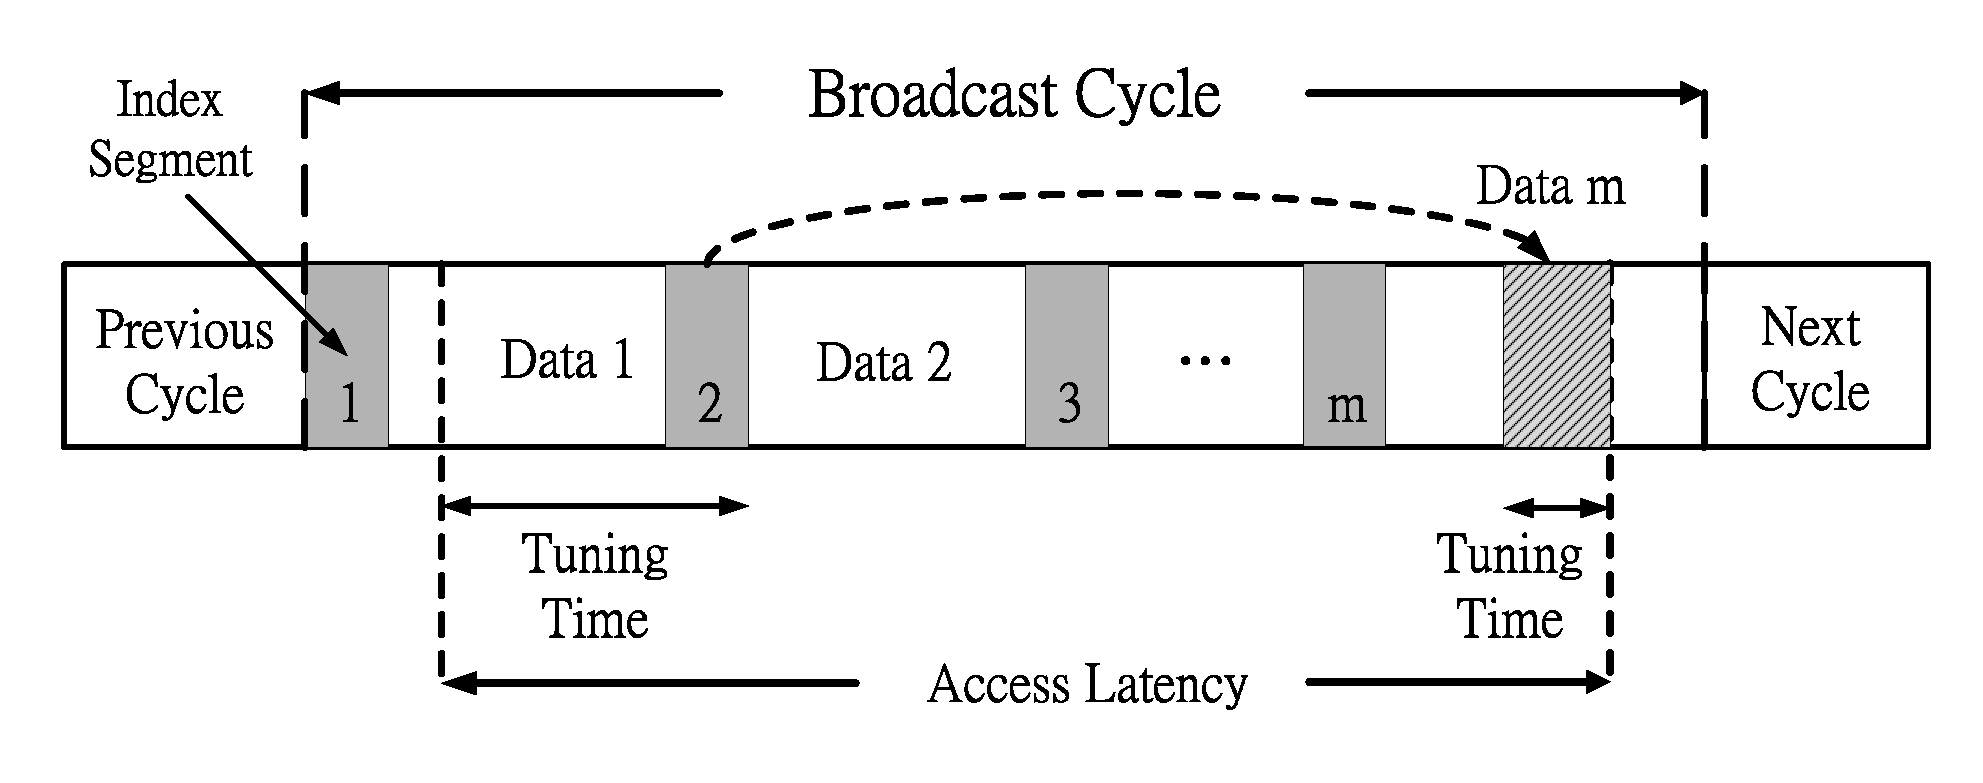
\includegraphics[width=4in]{Figures/BroadcastCycle.eps}
\vspace*{-15pt} \caption{Broadcast program cycles.}\vspace*{-10pt}
\label{fig:bcastcycle}
\end{center}
\end{figure}

Power consumption is a major concern in wireless broadcast
environments since most clients are mobile devices, such as
cellular phones, powered by a small battery. Therefore, power is a
scarce and valuable resource for these devices; continuously
listening to the broadcast channel is expensive in terms of power
usage. Most mobile devices are able to turn off the radio receiver
when they are not actively receiving data to conserve power. To
reduce power consumption, an index is used to make the broadcast
cycle self-descriptive. As depicted in
Figure~\ref{fig:index_node}, an index provides additional
information in a broadcast program to tell the clients the
approximate time that a data record will be broadcast. A broadcast
index is analogous to an index in traditional databases in which
the indexes provide the location of data records and facilitate
fast lookup of records. With the index information, the clients
can turn off the radio receiver to conserve power and only tune
into the channel when the desired data is being broadcast.

\begin{figure}[!h]
\centering \subfigure[Data set.]{

\includegraphics[width=2in]{Figures/mbr_2d.eps}
\label{fig:mbr_2d} } \subfigure[On air index.]{

\includegraphics[width=2in]{Figures/index_node_entry.eps}
}\vspace*{-10pt} \caption{A sample broadcast index.}
\label{fig:index_node}
\end{figure}

Adding an index to a broadcast cycle also adds space overhead to
the cycle and consumes broadcast bandwidth. Quantities that
measure the efficiency of a wireless broadcast program are defined
below. \emph{Access latency} and \emph{tuning time} are well-known
metrics of the broadcast model and have been studied
in~\cite{journals/vldb/ZhengLLLS09,journals/tkde/ImielinskiVB97,
conf/icde/KuZW07,journals/tmc/KuZW08,journals/winet/LeeL99}. We
also define \emph{index percentage} and \emph{initial index probe}
as measurements of index space overhead and index probe latency.

\begin{definition}[Access latency]\label{def:access_latency}
The amount of time from when a client requests data to the point
when the client receives all the desired data. This quantity is
denoted by $\alpha$.
\end{definition}

\begin{definition}[Tuning time]\label{def:tuning_time}
The total amount of time a client actively listens to the channel.
The time determines the power consumed by the client to retrieve
the required data. The quantity is denoted by $\tau$.
\end{definition}

Both the access latency and the tuning time are measured in terms
of number of data packets.

\begin{definition}[Index percentage]\label{def:index_percentage}
The ratio of the space allocated to the index to the space of the
entire cycle measures in bytes. This quantity is defined as $\rho
= \frac{\delta}{\omega}$.
\end{definition}

\begin{definition}[Initial index probe]\label{def:index_probe}
The amount of time for a client to get to the first index segment.
This quantity is denoted by $\lambda$.
\end{definition}


\begin{table}[!h]
\centering \caption{Summary of notations.} \vspace*{5pt}
\label{tab:index_attr}
\begin{tabular}{|c|p{2.45in}|}
\hline
{\bf Notation} & {\bf Description}\\
\hline\hline
$n$ & Number of dimensions of skyline \\
$m$ & Number of index segments in a cycle \\
$D$ & A set of attribute domains $D$ = \{$d_1$, ..., $d_n$\} \\
$T$ & A set of records (tuples) \\
%$p$ & A record (a n-tuple) \\
%$S$ & A set of skyline points \\
$\sigma$ & A set of skyline preference specifiers \\
%$R$ & A pruning region \\
$B$ & A minimal bounding box (MBR) \\
$E$ & An R-tree index entry (MBR, time) \\
$b$ & Branching factor of an index tree \\
$h$ & Height of an index tree \\
%$L$ & Tree level \\
$L_r$ & Levels of index tree replication \\
$\rho$ & Index percentage \\
%$\alpha$ & Initial index probe \\
$\alpha$ & Access latency \\
$\tau$ & Tuning time \\
$\delta$ & Size of a broadcast index \\
$\theta$ & Size of a broadcast data set \\
$\omega$ & Size of an entire program cycle $\delta + \theta$ \\
\hline
\end{tabular}
\end{table}

\begin{comment}
\begin{mydef}[Constraint Skyline] Give a set of spatial constraints
    $C$ = \{$c_1$, $c_2$, ..., $c_n$\}
    \begin{equation}
    ConsSkyline(P) = Skyline(P), \\where p \epsilon P~satisfies~C
    \end{equation}
\end{mydef}
\end{comment}


\section{Related Work}\label{sec-related}

\subsection{Skyline Computation}

Algorithms of the computation of skyline records in traditional database systems have been studied in~\cite{conf/icde/BorzsonyiKS01,shooting_stars,progressive_skyline}. The well-known algorithms are Nested-Loop, Block-Nested-Loop, and Divide and Conquer have studied in \cite{conf/icde/BorzsonyiKS01}. The Nested-Loop algorithm is a naive algorithm that it compare every record with every other record. In Block-Nested-Loop, a record is only compared with other records in the same block. In Divide and Conquer (D\&C) utilizes divide and merge strategy to computer skyline.

%\cite{shooting_stars} introduces an online skyline computation algorithm in which the skyline are computed progressively. The first skyline is returned almost immediately and more skyline points are added to the result set.

Branch-and-Bound Nearest Neighbor \cite{progressive_skyline} algorithm utilizes a tree index to efficiently computes skyline. In the design, data records are represented geometrically and a tree index is built on the data. The algorithm then uses branch-and-bound tree traversal to find nearest neighbors as skyline. Our algorithms uses a geometric tree index, but BBS-NN cannot be easily adopted to the broadcast environment due to that the algorithm requires backtracking of the tree.

%Nearest Neighbor (NN) and Branch-and-Bound (BBS) skyline algorithms are two of the best-performing algorithms for progressive skyline computation for traditional database systems presented in~\cite{progressive_skyline}. In the NN skyline algorithm, the records of the data set are presented geometrically in a Euclidean space with the relevant attributes as the coordinate in each dimension. In the example of a hotel close to the ocean previously presented, a record would be placed on a plane with the distance of the hotel to the ocean and its price as the two axes that determine its ranking, and the values in the two attributes as the coordinates of the records on the Euclidean plane. The NN algorithm finds a nearest neighbor from the axes; that is the first skyline point. Then the algorithm marks the region that is dominated by the first skyline point so that anything in that region will not be searched. The search results in two more search regions and the search continues until no more records are left.

%as in Figure~\ref{fig:skyline_nn}

%\begin{figure}[h]
%\begin{center}
%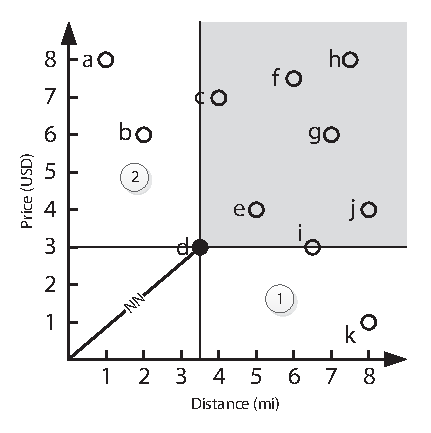
\includegraphics[width=2in]{Figures/skyline_nn.eps}
%\vspace*{-5pt} \caption{NN d and its pruning region.}
%\label{fig:skyline_nn} \vspace*{-10pt}
%\end{center}
%\end{figure}

%BBS is an algorithm that surpasses the computation efficiency of the NN algorithm. BBS utilizes the best first search technique to traverse the index tree to prune the unnecessary branches. Unfortunately, both NN and BBS cannot be easily adopted to the broadcast environment due to the linear nature of the broadcast program. Both NN and BBS require backtracking of the index tree to find the best path to prune (which is impermissible in the broadcast environment) or require waiting for the next broadcast cycle (which incurs a long waiting time). The solutions presented in this paper will use the pruning region strategy used in NN. Our algorithms systematically build pruning regions, as presented in the NN algorithm, as the client receives and discovers more data from the broadcast channel.

% SQL Operator
Extension SQL syntax for skyline was defined by B{\"o}rzs{\"o}nyi et al. in~\cite{conf/icde/BorzsonyiKS01}. The syntax defines an additional SKYLINE clause in SQL that specifies how the skyline operation should be performed. %In the SKYLINE clause, relevant attributes can be listed. For each attribute, the syntax defines three attribute specifiers, MIN, MAX, and DIFF, that tell the operator how each attribute is to be handled. MIN and MAX denote that the values of the attribute should be minimized or maximized; DIFF denotes that the values should be different.

\subsection{Wireless Broadcast Index}\label{sec:wireless_bcast_index}

%Many excellent studies have been done on improving the efficiency of wireless broadcast systems using indexing techniques. This section considers several popular index allocation techniques and discusses their benefits and drawbacks.

The intuitive technique of no index and one-time index at the beginning of a broadcast cycle has been considered in~\cite{journals/tkde/ImielinskiVB97}. With no index, the length of a cycle is minimized, but the tuning time is the entire cycle since the program is not self-descriptive. With one-time index, the clients are able to filter unwanted data and reduce tuning time, but if a client misses the one-time index, then it will have to wait until the next cycle even if there is useful data in current cycle.

$(1, m)$ indexing, proposed by Imielinski, \emph{et al.} in~\cite{journals/tkde/ImielinskiVB97}, is a mitigation to the problem of one-time index by replicating the entire index every $1/m$ length of the broadcast cycle. The benefit of this index technique is that when a client misses an index segment, it can wait for the next index in the same cycle~\cite{journals/tmc/KuZW08}. The drawback of this technique is the space consumption of replicating the full index several times in the cycle.

Distributed index was also proposed in~\cite{journals/tkde/ImielinskiVB97}. This index also replicates the index in the broadcast cycle, but only a part of the index is replicated. Advantages of this method are (1) an index can be obtained throughout a cycle, (2) reduced bandwidth consumption compared with $(1, m)$, and (3) the method is not limited to any particular index structure.

%\cite{data_on_air} by Imielinski, et al. is an
%early and influential work of data
%indexing for broadcast on air. The paper defined two
%characteristics of wireless broadcast, \em{tuning time} and \em{access latency}. Tuning time
%defines how long the client has to actively listen on the channel to get all the desired data.
%Access latency define the time when the client issues the query to the time all the desired
%data is received. Tuning time is proportional to power usage of mobile clients. The goal is to
%reduce both tuning time and access latency.

%In addition, the paper also proposed a few air index techniques to reduce client tuning time.
%The first index proposed is $(1, m)$ index, in which the full index is repeated every $1/m$ of
%the entire broadcast cycle. The index is repeat so that clients that tune into the channel in
%the middle of the broadcast does not have to wait until the next cycle to get the index and
%process request. The second index proposed is the distributed index, in which only a part of
%the index is repeated. Distributed index reduces the overhead of embedding index and improves
%access latency.

%Data filtering based on data signatures was proposed in~\cite{journals/winet/LeeL99}. During data retrieval, the signature of the desired data is compared with the signature of a data segment prepared by the broadcast server. If the signatures match, then the data is downloaded; otherwise it is ignored.
Distributed index for spatial data in error-prone air broadcast was introduced in~\cite{journals/vldb/ZhengLLLS09}. Instead of replication, this paper proposes a distributed index in the broadcast cycle with no duplicate indexes. The paper indexes broadcast spatial data using Hilbert values. Each data record contains an index table that includes the data segments that will be pushed onto the channel in the near future. %A drawback of this approach is the loss of spatial precision due to the use of the space filling curve as the index.


%\section{System Model}

%In our theoretical model, the system consists of the broadcast server and multiple clients. As
%discussed in section 2.1, the server periodically broadcast data in a specific channel. Any client
%that is interested in any of the data serviced by the server tunes into the channel to get the
%desire data. The server contains a set of records as illustrated in Figure 4.

%In this model, we assume a pure broadcast model in which all data are transmitted through downlink
%bandwidth and that there is not uplink bandwidth. Clients must tune into the channel as long as it
%takes to obtain all desire data. Apparently, in order to support efficient query, the server must
%provide data index so that the client can tune in only when the relevant data is to be broadcasted
%In addition, this model contains only one transmission channel. Index must be transmitted on the
%same channel as the data.


\section{Tree-based Distributed Index}\label{sec-index}

In this section we introduce how the index and data are allocated
on the broadcast channel to form the broadcast program. We
introduce a Tree-based Distributed Index (TDI), our index
allocation technique, which is based on the distributed index
allocation proposed in~\cite{journals/tkde/ImielinskiVB97}. The
benefits of a distributed index over other allocation methods will
be discussed in Section~\ref{sec:wireless_bcast_index}.

We utilize an R-tree~\cite{conf/sigmod/Guttman84} to index our
multi-dimensional data records. We assume that each node of an
R-tree consists of $b$ number of entries, $\{E_1, E_2, ... E_b\}$,
where $b$ is the branching factor, or the number of children at
each internal node, of the index tree, as illustrated by
Figure~\ref{fig:index_node}. Each entry contains a pointer to a
child index node (if the node is not a leaf node), or a pointer to
a set of data records (if the node is a leaf node). The pointer
contains the time when the child item will appear on the broadcast
channel. An advantage of utilizing the R-tree is that the indexed
broadcast data can be employed to support other spatial query
types, such as range~\cite{conf/pods/PagelSTW93} and $k$NN
queries~\cite{journals/tods/HjaltasonS99}.

\subsection{Broadcast Structure}

A broadcast program cycle is a linear representation of the index
tree and data and consists of \emph{index segments} and \emph{data
segments}. Index segments contain temporal pointers to either
another index segment or a data segment. Data segments contain
actual data records. Index and data segments are interleaved to
form a broadcast program. Each index segment is further divided
into smaller units called buckets. Buckets are logical independent
units that represent a portion of the tree index. The purpose for
buckets is that a client does not have to download an entire index
segment if it only needs a bucket.

In addition to a list of temporal pointers, each index bucket also
contains a pointer to the next index segment and a pointer to the
beginning of next broadcast cycle. The purpose of these pointers
is to direct the client to the next index segment in the case that
the client tunes in at the index bucket but is not interested in
the data pointed by the index.

To save bandwidth, data segments do not contain any index
information other than data records. The broadcast program
structure is illustrated in Figure~\ref{fig:index_packet}.

\begin{figure}[!h]
\begin{center}

\includegraphics[width=4in]{Figures/index_packet.eps}
\vspace*{-5pt} \caption{Broadcast program cycle format with index
segments and data segments.} \vspace*{-10pt}
\label{fig:index_packet}
\end{center}
\end{figure}

\subsection{TDI Allocation}

After indexing the data set with an R-tree, the next step is to
publish both data and index onto the linear broadcast channel. TDI
allocates space for index and data by performing a depth-first
traversal of the index tree as illustrated in
Figure~\ref{fig:index_struct}. In this process, the root index
node $A$ is first included in the cycle because it is first
traversed. Index node $B_1$ is then included in the program
followed by $C_1$, then the data items $D_1$ and $D_2$. We utilize
depth-first traversal of the index tree instead of breadth-first
traversal in our design because breadth-first traversal cannot
distribute the appropriate portion of index that exactly indexes
the data segment which follows it.

%When an index is replicated, only the MBRs that have not been
%broadcast are published; therefore the replication is not a
%complete replication of the index.

TDI replicates the top $L_r$ levels of the index tree $b$ times,
where the root node is considered level 0. Therefore, the
replication is not an entire path replication of the index. The
replication helps the clients get a broader picture of upcoming
broadcast items. Given $n_i$ to be the current index node to be
broadcast, if the level of $n_i$ is $L_r$ or less, then the parent
of $n_i$ is replicated. Otherwise the parent is not replicated. An
example is shown in Figure~\ref{fig:index_struct}; the root and
the second level index nodes are replicated. Of course, the best
view of upcoming data records would be to replicate the entire
index, but this would be a complete replication, which we try to
avoid to decrease broadcast cycle length.

\begin{figure}[!h]
\begin{center}

\includegraphics[width=5in]{Figures/bcast_struct.eps}
\caption{Index Structure.} \vspace*{-10pt}
\label{fig:index_struct}
\end{center}
\end{figure}

%and $\varepsilon$ be the space required for an index node entry

\subsection{Analysis}

This section presents the derivation of the two performance
evaluation metrics of the tree-based distributed index, which we
defined in Subsection~\ref{sec:wireless_broadcast}.

\subsubsection{Index Percentage}

Index percentage measures the space overhead of the index
structure. It is defined as the ratio between the space allocated
to the index on the broadcast cycle to the length of the entire
broadcast cycle.

Let $L_r$ be the levels of replication (for example, $L_r$ for the
TDI in Figure~\ref{fig:index_struct} is 2) and $\eta$ be the space
required for an index node. The number of nodes replicated in the
cycle is $(\displaystyle\sum\limits_{i=0}^{L_r-1} b^i)$. In TDI,
each replicated index node appears $b$ times in one cycle.
Consequently, the total space taken by the index is the space for
all index nodes plus the additional space for replication. It is
given by:

\begin{equation}
\delta = \eta\{(\displaystyle\sum\limits_{i=1}^{h-1} b^i + 1) +
(\displaystyle\sum\limits_{i=0}^{L_r-1} b^i)(b - 1)\}
\end{equation}

The length of the broadcast cycle $\omega$ is the space of the
index plus the space of the data ($\delta+\theta$). Therefore, the
index percentage is defined as:

\begin{equation}
\rho = \frac{\delta}{\omega}
\end{equation}

\subsubsection{Initial Index Probe}

The tree-based distributed index divides the entire data set into
smaller data segments and reduces the initial probe of the first
index segment. The length of each data segment, denoted by $\ell$,
is determined by the number of index segments distributed among
the broadcast cycle. As one can see in
Figure~\ref{fig:index_struct}, there are four leaf nodes in the
index and the data is divided into four segments. Therefore, the
number of data segments is $b^{L_r}$ and the size per data segment
is:

\begin{equation}
\ell = \frac{\theta}{b^{L_r}}
\end{equation}

The initial index probe is half of the length of an index segment
plus a data segment:

\begin{equation}
\lambda = \frac{1}{2}(\frac{\delta}{b^{L_r}}+\ell)
\end{equation}

%This is a significant time reduction compare with one-time index
%probe.

%\subsection{Motivation for DFDI}
%Consider that we have an R-tree to index our multi-dimensional data, we
%need to consider the broadcast structure and format so that the index
%and data packets can be broadcasted on the same channel. Tree index
%structures are of particular interest since trees are non-linear whereas
%broadcast program is strictly linear.

%Given two sibling index nodes $A$ and
%$B$ and their parent index node $P$, the following rules determine if
%an index node is replicated in the broadcast program:
%
%\begin{enumerate}
%\item If $A$ is the current index, and $P$ is part of the replicated
%        portion of the index, then $A.ind\_ptr$ points to an index packet
%        and segment that contains both $P$ and $B$.
%\item If $A$ is the current index, and $P$ is \emph{not} part of the
%        replicated portion of the index, then $A.ind\_ptr$ points to
%        an index packet (or segment) that contains only $B$.
%\end{enumerate}

%The broadcast algorithm based on our tree-based distributed index
%is formalized in Algorithm~\ref{alg:TDI}.
%
%\begin{algorithm}
%\algsetup{linenosize=\small,linenodelimiter=. }
%\caption{TDI($Node$, $Level$, $L_r$)} \label{alg:TDI}
%\begin{algorithmic}[1]
%
%\STATE PushToChannel($Node$) \COMMENT{Assume temporal ptrs are
%known} \IF{$Node$ is Leaf}
%    \FORALL{DataSegment in $Node$}
%        \STATE PushToChannel(DataSegment)
%    \ENDFOR
%\ELSE
%    \FORALL{ChildNode in $Node$}
%        \STATE TDI(ChildNode, $Level$++)
%        \IF{$L_r$ $\leq$ $L$ AND NOT Last ChildNode}
%            \STATE PushToChannel($Node$)
%            \COMMENT{Replication}
%        \ENDIF
%    \ENDFOR
%\ENDIF
%\end{algorithmic}
%\end{algorithm}


\section{Pruning Region Broadcast Skyline}\label{sec-pruning}
In this section, we present skyline computation algorithms. We first describe the concept of a pruning region, on which our algorithms are built. After foundations, two skyline algorithms are presented: Record-Based Pruning Skyline (RPS) is presented in Section~\ref{sec-RPS} and Index-Based Pruning Skyline (IPS) is presented in Section~\ref{sec-IPS}. Both RSP and IPS utilize the tree-based distributed index described in the previous section to build a set of pruning regions to eliminate unwanted data records. IPS generally provides better performance, but only produces correct result when the bounding boxes of the index tree does not overlap; whereas RSP works for any tree index.

The rest of this section describes pruning region. In the following definitions, when we say a point, $q$, and region, $R$, we mean a point and region in the data space such that ($q_1$, ..., $q_n$) are record attributes.

%In addition, to simplify our demonstration, we first consider 2-dimensional skyline. Later we show how our approach can be easily extended to higher dimensions.

%\begin{definition}[Pruning Region]
%Given the data space defined by $d_1 \times d_2 \times ... \times d_n$, where $d_i$ is the domain of attribute $i$, a pruning region is a pair of a pivot point and an ordered list of preference specifiers $(p, \sigma)$ that specifies a region of the data space that has been dominated by a subset of the data set. As defined in Section~\ref{sec-prelim}, $\sigma_i$ is one of the values in $\{min, max\}$.
%\end{definition}

\begin{definition}[Pruning Region]
A pruning region, $R$($d$, $\sigma$), is a rectangular region of data space that is dominated by one or more data records. $d$ is a point called dominant point and $\sigma$ is an ordered list of preference specifiers.
\end{definition}

Given an arbitrary point $d$ and $\sigma$, a pruning region $R$ is defined such that for each attribute $i$, if $\sigma_i = min$, then $d_i$ is the lower bound of $R$ for the $i$th dimension and the region extends to the maximal value for the $i$th dimension. Similarly, if $\sigma_i = max$, then $d_i$ is the upper bound and extends to minimal value of the dimension.

A dominant point can also be defined with any rectangle as follows:

\begin{definition}[Dominant Point]\label{def-dominant-point}
Given a n-dimensional rectangle, $B$, and a list of skyline preference specifiers, $\sigma$, the dominance point of the rectangle $d$($B$, $\sigma$) is the point of intersection of all axes of the data space and contains the ``best" of all axes in $B$, where the ``best" is defined by $\sigma$.
\end{definition}

The ideas of dominant point and pruning region are illustrated in Figures~\ref{fig:rtree_pr} where pruning regions are illustrated as the gray regions and dominant points are solid dots. The figure shows a 2-dimensional (Figure~\ref{fig:rtree_pr_2d}) and a 3-dimensional (Figure~\ref{fig:rtree_pr_3d}) data space with 2 pruning regions defined by dominant points $b$ and $d$. As illustrated, a pruning region is a region of an n-dimensional space that has been dominated by pivot point and can be ignored in the upcoming broadcast data stream.
By Definition~\ref{def-dominant-point}, we have the following properties:

\begin{property}\label{property:record_pruning}
Given $\sigma$, a pruning region can be constructed from any arbitrary data record, $p$, as $R$($p$, $\sigma$).
\end{property}

\begin{property}\label{property:pivot_point}
The dominant point of pruning region $R$ dominates all data points and minimal bounding rectangles inside $R$.
\end{property}

\begin{figure}[!h]
\centering
\subfigure[2-D space with $\sigma$ = ($min$, $min$).]{

\includegraphics[width=2.2in]{Figures/rtree_pr2.eps}\label{fig:rtree_pr_2d}}
\subfigure[3-D space with $\sigma$ = ($min$, $min$, $max$).]{

\includegraphics[width=2.2in]{Figures/rtree_pr_3d.eps}\label{fig:rtree_pr_3d}}
\caption{Pruning region with candidate Skyline points.\label{fig:rtree_pr}}
\end{figure}

Our skyline algorithms utilize pruning regions to determine if a record (a point in data space) or a branch of the index (a bounding rectangle) from the broadcast program can be ignored. The data items (record or index) that can be ignored are the ones that are covered by (or inside) any of the pruning regions that the skyline algorithm constructs and maintains. The following lemma determines if a data record covered by a pruning region.

\begin{lemma}\label{lemma:point_covered}
A data record, $p$, is covered by a pruning region $R$($d$, $\sigma$), if for each attribute $i$, one of the following is met:
\begin{enumerate}
  \item If $\sigma_i$ = $min$, then $p_i \geq d_i$
  \item If $\sigma_i$ = $max$, then $p_i \leq d_i$
\end{enumerate}
\end{lemma}

Lemma~\ref{lemma:point_covered} says to check if a data record, $p$, is covered by a pruning region, all attributes of the record has to be compare against the dominant point(or record), $d$, of the pruning region. If any attribute does not satisfy any of the two conditions, the record is not covered.

To determine if a branch of the broadcast index is covered by a pruning region, we need to compare the minimal bounding box of the index branching to the pruning region. By Property~\ref{property:pivot_point}, the following determines if a rectangle (bounding box) is covered.

\begin{lemma}\label{lemma:rect_covered}
Given a pruning region $R$($d$, $\sigma$) and a rectangle $B$, $R$($d$, $\sigma$) covers $B$ if $R$($d$, $\sigma$) covers the dominant point of $B$, $d$($B$, $\sigma$).
\end{lemma}

\begin{proof}
The pruning region $R$($d$, $\sigma$) covering the dominance point $d$($B$, $\sigma$) of $B$ implies that one of the conditions of Lemma~\ref{lemma:point_covered} is true for every attribute and that $d$ $\succ$ $d$($B$, $\sigma$). Due to Property~\ref{property:pivot_point}, $d$ $\succ$ $B$.
\end{proof}

An example is given in Figure~\ref{fig:pruning}. A pruning region $R$($s$, $\sigma$) is illustrated in gray with $\sigma$ = ($X$ = $min$, $Y$ = $max$). Bounding box $A$ can be pruned since its dominant point, $d$($A$, $\sigma$), falls inside the pruning region, while bounding box $B$ cannot be pruned since, although it is partially covered, its dominant point,  $d$($B$, $\sigma$), does not fall inside the pruning region.

\begin{figure}
\begin{center}

\includegraphics[width=3in]{Figures/pruning.eps}
\vspace*{-5pt} \caption{A pruning region defined by $d$ and
$\sigma$ = $(X = min, Y = max)$.} \vspace*{-5pt}
\label{fig:pruning}
\end{center}
\end{figure}



\subsection{Record-Based Skyline Pruning}\label{sec-RPS}

In this section, we present our skyline algorithm that utilizes the data records received from the broadcast program to construct pruning regions. At the beginning of the algorithm, the list of pruning regions, maintained by the algorithm, is empty. At this state, the algorithm cannot prune any broadcast item (index or data); therefore stays tuned into the channel and follows the index to the first data segment. As the algorithm receives data records, it constructs one pruning region for each data record as state in Property~\ref{property:record_pruning}. The following summarizes the notations we use in algorithm listings:

\begin{table}[!h]
\centering \caption{Algorithmic Notations}\label{tab:alg}
\begin{tabular}{|c|p{2in}|}
\hline
{\bf Symbol} & {\bf Description}\\
\hline\hline
$S$ & A set of candidate skylines; $S'$ denote local skylines.\\
$R$ & A set of pruning regions; $R'$ denotes local pruning region.\\
GetBucket($E$) & Wait and download items specified by $E$. \\
Skyline($B$, $\sigma$) & Compute skyline from set $B$ via NN. \\
GetPRegions($S$, $\sigma$) & Compute pruning regions from set $S$. \\
Prune($S$, $R$) & Remove items from $S$ that are covered by $R$.\\
\hline
\end{tabular}
\end{table}

The RPS algorithm is shown in Algorithm~\ref{alg:RBSkyline}. During initialization (line 1-2) of the algorithm, the list of candidate skylines, $S$, and the list of pruning regions, $R$, are assigned the empty set.

After initialization, the algorithm goes into the outer loop (line 3-32) that iterates through all branches of the index tree. For the first iteration, the first index bucket is downloaded (line 5-6). If the bucket is the root node of the index, then there is no sibling branch and $next$ remains $null$; otherwise, $next$ is set to the time of the next index segment(line 10-12), which contains the next branch.

In the inner loop (line 13-31), the algorithm pops the next data item, a bucket, to be downloaded, and downloads the data item (line 15). If the bucket downloaded is index, then each index entry, expressed as ($mbr$, $time$) pair, is push onto the stack (line 17-22). If bucket is not index, but is data, then the following are performed (line 23-30).

\begin{enumerate}
\item Computes local skyline, $S'$, of the data bucket (line 24).
\item Computes local pruning regions, $R'$, from $S'$ (line 24).
\item Prune records in $S$ and stack entries covered by $R'$ (line 26-27).
\item Add (union) local pruning regions, $R'$, to global regions, $R$ (line 28).
\item Add (union) local skyline,$S'$, to global skyline, $S$ (line 29).
\end{enumerate}

Note that $S$ are candidate skyline since there could be data objects broadcast later that dominate the earlier candidate Skyline points. For example, if a later candidate point $s'$ dominates an earlier point $s$, then $s$ is removed from $S$ and the pruning region is enlarged by the later point $s'$.

The skyline computation phase ends when the stack is empty and $S$ is returned as skyline (line 33).

\begin{algorithm}[!h]
\algsetup{linenosize=\small,linenodelimiter=. }
\caption{Record-Based Skyline($\sigma$)} \label{alg:RBSkyline}
\begin{algorithmic}[1]

\STATE $S$ $\gets$ $\emptyset$
\STATE $R$ $\gets$ $\emptyset$
\REPEAT
    \STATE next $\gets$ null
    \IF {first iteration}
        \STATE bucket $\gets$ search first index bucket
    \ELSE
        \STATE bucket $\gets$ GetBucket(next)
    \ENDIF

    \IF {\NOT IsRootNode(bucket)}
        \STATE next $\gets$ bucket.time\_of\_next\_index\_segment
    \ENDIF

    \WHILE {\NOT stack.empty \OR first iteration}
        \IF {not first iteration}
            \STATE bucket $\gets$ GetBucket(stack.pop)
        \ENDIF
        \IF {IsIndex(bucket)}
            \FOR {$E_i$ in bucket, $i$ = $b$ to 1}
                \IF {\NOT Covers(R, $E_i$)}
                    \STATE stack.push($E_i$)
                \ENDIF
            \ENDFOR
        \ELSE
            \STATE $S'$ $\gets$ Skyline(bucket, $\sigma$)
            \STATE $R'$ $\gets$ GetPRegions($S'$, $\sigma$)
            \STATE Prune($S$, $R'$)
            \STATE Prune(stack, $R'$)
            \STATE $R$ $\gets$ $R$ $\cup$ $R'$
            \STATE $S$ $\gets$ $S$ $\cup$ $S'$
        \ENDIF
    \ENDWHILE
\UNTIL{next = null}
\RETURN $S$
\end{algorithmic}
\end{algorithm}


\subsection{Index-Based Skyline Pruning}\label{sec-IPS}

The drawback of the RPS is that the algorithm has to receive data records before pruning regions can be formed. In this section we present index-based pruning skyline (IPS) that utilizes the index bounding boxes to form pruning regions. The expectation is that the index usually precede data records. If we can make pruning regions early using index, then more of the index tree could be pruned. Note that this algorithm only produces correct result when the bounding boxes, of the same level of the index tree, do not overlap, such as index structures described in \cite{DBLP:conf/vldb/SellisRF87}\cite{DBLP:journals/acta/FinkelB74}\cite{DBLP:conf/compgeom/Bentley90}. We define the follow definition and theorem to formulate IPS:

%The reason we only use data records as criteria to form pruning region to accommodate overlapping region in index tree (such as in R-Tree).

%One of index structure that supports non-overlapping index regions is R+-Tree which can be found in ~\cite{DBLP:conf/vldb/SellisRF87}.

\begin{definition}[Anti-Dominant Point]\label{def:anti-dominant-point}
Given a n-dimensional rectangle, $B$, and a list of skyline preference specifiers, $\sigma$, the anti-dominance point of the rectangle $ad$($B$, $\sigma$) is the point of intersection of all ``worst" bounds of $B$, where the ``worst" is defined by $\sigma$.
\end{definition}

\begin{theorem}\label{theorem:IPS}
Given that bounding boxes on the same level of the index do not overlap and the following:
\begin{itemize}
  \item A n-dimensional minimal bounding box, $B$
  \item Skyline preference, $\sigma$
  \item Dominant point of $B$, $d$ = $d$($B$, $\sigma$) = ($d_1$, $d_2$, .., $d_n$)
  \item Anti-dominant point of $B$, $a$ = $ad$($B$, $\sigma$) = ($a_1$, $a_2$, .., $a_n$)
\end{itemize}
a set of n pruning regions, $R$, can be created from $B$, as
\begin{equation}
R_B = \{R((a_1, d_2, .., d_n), \sigma), R((d_1, a_2, .., d_n), \sigma), .., R((d_1, d_2, .., a_n), \sigma)\}
\end{equation}
\end{theorem}

\begin{proof}
According to the definition of minimal bounding box~\cite{DBLP:journals/gis/PapadiasT97}, for each bound of $B$, there must be a point that defines that particular bound, such that there is a set of points, $P$ = \{$p_1$, $p_2$,.., $p_m$\} $m \leq 2 \times n$, that defines $B$. By Property~\ref{property:record_pruning}, a set of pruning regions can be created for each point in $P$, $R_P$ = \{$R$($p_1$, $\sigma$), $R$($p_2$, $\sigma$), .., $R$($p_m$, $\sigma$)\}. Since $R_B$ is created from the anti-dominant point of $B$, $R_P$ completely covers $R_B$.
\end{proof}
%\begin{proof}
%Here we provide a proof for a two-dimensional case. Given the following:
%\begin{itemize}
%  \item A minimal bounding box, $B$, defined by two corner points of $B$: $lower$ = ($l_1$, $l_2$), and $upper$ = ($u_1$, $u_2$).
%  \item $\sigma$ = ($min$, $min$)
%\end{itemize}
%
%There must exist at least one point, $p$ = ($p_1$, $p_2$), in $B$ such that $p_2 = B.l_2$, $p_1$ $\epsilon$ [$B.l_1$, $B.u_1$]. Similarly, there must exist another point, $q$ = ($q_1$, $q_2$) such that $q_1 = B.l_1$, $q_2$ $\epsilon$ $[B.l_2, B.u_2]$.
%
%$p$ dominates anything to the right of $p_1$ and above $B.min_2$ and $q$ dominates all records above $q_2$ and to the right of $B.min_2$. We extend the $p_2$ value of the pruning region of $p$ and the $q_1$ value of the pruning region of $q$ and these two are the same as the values for the pruning region of point $(B.min_1, B.min_2)$. Since MBRs do not overlap, pruning regions for point $(B.min_1, B.min_2)$ is the pruning region of the MBR $B$.
%\end{proof}

Theorem~\ref{theorem:IPS} states that for each minimal bounding box, $B$, of the index that we have examined, a set of $n$ pruning regions, $R_B$, is created. We can improve memory usage slightly by merging all pruning regions in $R_B$ and create only one, $R_m$ = $R$($d$($B$, $\sigma$), $\sigma$)), to keep in memory. Not only does $R_m$ cover $R_B$, but it also covers the entire $B$; therefore, if this optimization is used, the algorithm must keep track that $B$ should still be considered for skyline computation if it had not already visited.

We term the original n-region and the optimization one-region strategies. Figure~\ref{fig:ibp_a} illustrates the one-region strategy in which one pruning region is created from minimal bounding box $A$. Note that $A$ is inside the pruning region, but should still be visited. Figure~\ref{fig:ibp_b} illustrates n-pruning regions created from $A$. $n$ always equals the dimensionality of the data, in this case $n$ = 2. Our algorithm implements the n-region strategy described by the theorem.

\begin{figure}[!h]
  \centering
  \subfigure[Pruning with one Pruning Region]{
    \label{fig:ibp_a}
    %\begin{minipage}[h!]{0.5\textwidth}
      
\includegraphics[width=2.5in]{Figures/index_based_pruning_a.eps}
    %\end{minipage}
    }
  \subfigure[Prune with $n$ Pruning Regions]{
    \label{fig:ibp_b}
    %\begin{minipage}[h!]{0.5\textwidth}
      
\includegraphics[width=2.5in]{Figures/index_based_pruning_b.eps}
    %\end{minipage}
    }
  \caption{Index-Based Pruning Strategies (min, min)}
  \label{fig:ibp}
\end{figure}

IPS is shown in Algorithm~\ref{alg:IBSkyline}. The initialization and outer loop is the same as RPS. During skyline computation phase (line 13-30), the next expected item (index or data bucket) is popped from the stack and downloaded from the channel. If the item is an index, then each inner (bounding box, broadcast time) pair is checked to see if $R$ covers the bounding box (line 9). If the bounding box is not covered, then the pair is pushed onto the stack, and $n$ pruning regions are computed as follows:

\begin{enumerate}
\item The next level bounding box is pushed onto the stack to be downloaded in future iteration (line 20).
\item The local pruning region, $R'$ is computed from the next level bounding box (line 21).
\item Candidate skyline and queue entries that are covered by $R'$ are removed (line 22-23).
\item Local pruning regions, $R'$, is added to the global pruning regions (line 24).
\end{enumerate}

If the downloaded item is a data bucket, then skyline is computed from the bucket and added to the set of candidate skyline (line 28). As in RPS, when the stack is empty, $S$ is returned as skyline result.

\begin{algorithm}[!h]
\algsetup{linenosize=\small,linenodelimiter=. }
\caption{Index-Based Skyline($\sigma$)} \label{alg:IBSkyline}
\begin{algorithmic}[1]

\STATE $S$ $\gets$ $\emptyset$
\STATE $R$ $\gets$ $\emptyset$
\REPEAT
    \STATE next $\gets$ null

    \IF {first iteration}
        \STATE bucket $\gets$ search first index bucket
    \ELSE
        \STATE bucket $\gets$ GetBucket(next)
    \ENDIF

    \IF {\NOT IsRootNode(bucket)}
        \STATE next $\gets$ bucket.time\_of\_next\_index\_segment
    \ENDIF

    \WHILE{\NOT stack.IsEmpty \OR first iteration}
        \IF {not first iteration}
            \STATE bucket $\gets$ GetBucket(stack.pop)
        \ENDIF
        \IF {IsIndex(bucket)}
            \FOR {$E_i$ in index, $i$ = $b$ to 1}
                \IF {\NOT Covers(R, $E_i$)}
                    \STATE stack.push($E_i$)
                    \STATE $R'$ $\gets$ GetPRegions(e.mbr, $\sigma$)
                    \STATE Prune($S$, $R'$)
                    \STATE Prune(stack, $R'$)
                    \STATE $R$ $\gets$ $R$ $\cup$ $R'$
                \ENDIF
            \ENDFOR
        \ELSE
            \STATE $S$ $\gets$ $S$ $\cup$ Skyline(bucket, $\sigma$)
        \ENDIF
    \ENDWHILE
\UNTIL {next = 0}
\RETURN $S$
\end{algorithmic}
\end{algorithm}

%\begin{algorithm}
%\algsetup{linenosize=\small,linenodelimiter=. }
%\caption{ComputePruneRegion($S$, $\sigma$)}
%\label{alg:ComputePruneRegion1}
%\begin{algorithmic}[1]
%
%\STATE $totalR \gets$ \o \FORALL{$p$ in $S$}
%    \STATE $tempR \gets$ ($-\infty$ to $\infty$) for all dimensions
%    \FOR{$i = 0$ to $n$}
%        \IF{$\sigma[i] = MIN$}
%            \STATE $tempR \gets tempR \bigcap (\infty \bigcup ... \bigcup (s[i]~to~\infty)_i \bigcup ... \bigcup \infty $)
%        \ELSE
%            \STATE $tempR \gets tempR \bigcap (\infty \bigcup ... \bigcup (min(D_i)~to~s[i])_i \bigcup ... \bigcup \infty $)
%        \ENDIF
%    \ENDFOR
%    \STATE $totalR \gets totalR \bigcup tempR$
%\ENDFOR \RETURN $totalR$
%\end{algorithmic}
%\end{algorithm}


%\begin{algorithm}
%\algsetup{linenosize=\small,linenodelimiter=. }
%\caption{ComputePruneRegion($B$, $\sigma$)}
%\label{alg:ComputePruneRegion2}
%\begin{algorithmic}[1]
%\STATE $R \gets$ \o \FOR{$i = 0$ to $n$}
%    \IF{$\sigma[i] = MIN$}
%        \STATE Add dimension $i$ to $R$ from 0 to $\infty$
%    \ELSE
%        \STATE Add dimension $i$ to $R$ from 0 to $B.i_{max}$
%    \ENDIF
%\ENDFOR \RETURN $R$
%\end{algorithmic}
%\end{algorithm}

%\subsubsection{Data Preparation}
%The data and index preparation is the same as in Solution1. The only difference is that instead
%of indexing the data with R-Tree, this solution index the data with R+-Tree. The attractiveness of
%this index structure is non-overlapping MBR and we can quickly find the pruning region in our
%algorithm. Give an example of why overlapping would cause a problem.

%A drawback of this index technique is creating an R-Tree without overlapping MBRs incur
%computational overhead (cite).


%\subsubsection{Skyline Computation}
%
%We start with pruning region that covers space. As soon as our algorithm receives the first index
%segment we get a sense of the data distribution in space we can start forming pruning regions.
%Consider example [provide example and attach figure].  The entire index tree consists of MBRs
%A and B. Let $Min(MBR)$ be the corner of MBR that has minimum of all dimension and $Max(MBR)$
%be the corner that has maximum of all dimension. Since $Min(B)$ < $Min(A)$, we can immediately
%form the pruning region, and prune MBR A.

%Note, we don't need to consider sub-MBRs inside A and B. Since the MBRs do not overlap, the
%entire region cover by A is dominated by B. Comparing with Solution 1, we don't have to traverse
%the tree to the leaf nodes to start forming pruning regions; instead, we can obtain pruning regions
%as early as the root node of the index. This has improvement in tuning time.


%\subsubsection{Correctness Verification}

%We consider the correctness of this algorithm for the MIN $x$, MIN
%$y$ case. This verification can be easily applied to other cases
%with combinations of attribute specifiers. Our goal is to prove
%the correctness of our index-based pruning algorithm. We want to
%show that we can form pruning regions from the MBR of an index
%node instead of wait until we receive data records as in
%Algorithm~\ref{alg:PBSkyline}. We also want to show that this
%algorithm does not prune false negatives (more than it should
%prune).
%
%We can form pruning region from the MBR of the index because the
%MBR of R+-Tree does not overlap. As we mentioned earlier in this
%paper, this technique does not work for index structures that
%allow overlapping index regions such as R-Tree and R*-Tree
%\cite{Beckmann:1990:RER:93597.98741}.
%
%Given a MBR, $b$, of data index that encloses data records, the
%$b$ is bounded by two points $(x_{min}, y_{min})$, $(x_{max},
%y_{max})$ and these points denote the lower-left and upper-right
%corners of the MBR respectively. There must exist a point, $p_1$,
%in $b$ such that $p_1.y = b.y_{min}$, $p_1.x$ in range
%$[b.x_{min}, b.x_{max}]$. Similarly, there must exist another
%point, $p_2$ such that $p_2.x = b.x_{min}$, $p_2.y$ in range
%$[b.y_{min}, b.y_{max}]$.
%
%$p_1$ dominates anything to the right of $p_1.x$ and above
%$b.y_{min}$ and $p_2$ dominates all records above $p_2.y$ and to
%the right of $b.x_{min}$. We extend the $y$ value of the prune
%region of $p_1$ and the $x$ value of the pruning region of $p_2$
%and these two are the same as the values for the pruning region of
%point $(b.x_{min}, b.y_{min})$. Since MBRs do not overlap, pruning
%regions for point $(b.x_{min}, b.y_{min})$ is the pruning region
%of the MBR $b$.

%\subsection{Skyline of Higher-Dimension}
%For skyline queries that involves more than two query attributes,
%we need to consider computation of skyline of higher dimension.
%Due to the generic nature of our algorithm, we can extend our
%algorithm to higher dimensions.
%
%Similar to skyline in two-dimension, we first need to index our
%data in an index structure. R-Tree and other spatial index
%structure, such as KD-Tree, can support data of arbitrary
%dimension. KD-Tree and Quad-Tree are better choice here due to
%lower computation complexity of building the index for
%higher-dimensional data. %We build our index as illustrated in Figure \ref{fig:rtree3d}.

%\begin{figure}[h]
%\begin{center}
%\includegraphics[width=3in]{Figures/rtree3d-eps-converted-to.pdf}
%\caption{\small Data Records inserted into R-Tree.\label{fig:rtree3d}}
%\end{center}
%\end{figure}

%Using the index, we can compute higher-dimensional pruning region
%(space) to facilitate skyline computation.

\subsection{Analysis}

In this section we consider tuning time and access latency of the
two pruning region skyline algorithms we presented in this
section. We assume that the client makes skyline queries at the
beginning of a cycle. Since the amount of time spent listening to
the channel is the amount of time required for a client to get all
the desired data, the tuning time is equal to access latency;
therefore, we use the same analysis for both quantities.

We first consider the tuning time for the algorithm that uses the
record-based pruning strategy. The best case is that the client
gets all desired data from the first data segment, and the rest of
the cycle is pruned. In this case, $\beta = h \times \eta +
\varsigma$. The expected case is when the client has to listen to
half of the program and $E(\beta) = \frac{1}{2}(\iota + \theta)$

We now consider the same quantity for the index-based pruning
skyline algorithm. The assumption is the same as before, but a
client does not have to traverse the index to the leaf level
before they start pruning. On average, a client would have to
traverse half of the index tree but would still have to download
half of the data; therefore $E(\beta) = \frac{1}{4}\iota +
\frac{1}{2}\theta$

%\subsubsection{No Index}
%
%When no index is added to the broadcast cycle, the program
%length is equal to the number of data packets. The tuning time, $t_t$
%and access latency, $t_l$, is also equal to program length since a client
%have to listen to the entire broadcast cycle to compute the skyline.
%
%\begin{equation}
%    l_p = t_t = t_l = d
%\end{equation}
%
%The initial index probing time and the index percentage do not apply
%and we set both to 0.
%
%\begin{equation}
%    t_p = p_i = 0
%\end{equation}
%
%\subsubsection{One-time index}
%
%In one-time index, the index packets only appear one time at the
%beginning of the program without replication. Consider every node
%is pack in one index packet. For a full R-Tree
%index, the following defines the relationship:
%
%\begin{eqnarray}
%% \nonumber to remove numbering (before each equation)
%  h &=& \log_{b} n_t - 1 \\
%  n_i &=& \displaystyle\sum\limits_{i=0}^h b^i \\
%  l_p &=& d + n_i
%\end{eqnarray}
%
%The expected tuning time and access latency is the half of the
%broadcast program:
%
%\begin{eqnarray}
%% \nonumber to remove numbering (before each equation)
%  t_t &=& \frac{1}{2} (d + n_i) \nonumber \\
%      &=& \frac{1}{2} (d + \displaystyle\sum\limits_{i=0}^h b^i) \\
%  t_l &=& t_t
%\end{eqnarray}
%
%\subsubsection{DFDI}
%
%Assume r percent of the index is replicated and the rest is not
%replicated, the program length is as follows:
%
%\begin{equation}
%    l_p = d + (1 + r) \displaystyle\sum\limits_{i=0}^h b^i
%\end{equation}
%
%The expected tuning time and access latency is the same as for the
%one-time index that is the half of the length of the broadcast
%program. Note that, even though, the function of these two metrics
%are the same, the program length is different for both cases.
%For DFDI, since we replicated $r$ percent of the index, the program
%length is longer, therefore, the latency and tuning time are also
%longer.

%The formulation of a pruning region depends on a pivot point, here we denote
%it with $p$, and the preference specifiers
%of the attributes of the data. For each axis (attribute) of the data space,
%the preference could be either MIN or MAX. For an axis $i$ with MIN specifier,
%the pruning space is from $p.i$ to $\infty$ (or maximum value for the attribute).
%Similarly, for the axis with MAX specifier, the pruning space is from $p.i$ to
%$-\infty$ or minimum value of the attribute. For data of positive value, the
%minimum value would be 0.


\section{Experimental Evaluation}\label{sec-exp}
In this section, we report our simulation results and evaluate the efficiency of TDI (our program allocation algorithm) and point-based and index-based skyline computation algorithms discussed in previous sections of this chapter. Our simulations are implemented in C\# with .NET Framework 4 (compatible with version2) and conducted on a machine of 3.4 GHz Intel Pentium 4 processor, 3 GB RAM, and Windows 7.

The simulations are ran with synthetic data-sets categorized as follows:

\begin{itemize}
\item Uniformed: data uniformly distributed in the data space of each
    attribute.
\item Rising: the attributes of the records are correlated to the first
    attribute of the data-set.
\item Falling: the attributes of the records are inversely correlated to
    the first attribute of the data-set.
\end{itemize}

In addition, we also conducted simulations of data-sets with varying \emph{record count} and \emph{dimensions}.  Record count ranges from 20,000 to 100,000, and dimensions ranges from 2 to 10. Our simulation are memory-only: at the started of a simulation, a data-set is loaded into memory from disk. Table~\ref{tab:sim_size} lists the size of data elements used in the implementation of the tuning time and index percentage simulation.

\begin{table}[h]
\caption{Simulation parameters.}
\label{tab:sim_size}
\centering
\begin{tabular}{l|c}
\hline
{\bf Item} & {\bf Size in Bytes}\\
\hline
Pointer of index ($ptr$) & 4\\
Field of record ($f$) & 8\\
Record/point ($p$) & $f \times n$\\
Minimal bounding rectangle (MBR) & $2 \times p$\\
Index entry ($E$) & MBR + $ptr$\\
\hline
\end{tabular}
\end{table}

\subsection{Dominance Tests}\label{sec:exp_dom_test}

\emph{Dominance tests} measures the number of record comparisons the client has to perform to evaluate a skyline query via Block-Nested-Loop (BNL)~\cite{conf/icde/BorzsonyiKS01}. A comparison determines if a record dominates another record. Comparisons are performed when a data bucket is downloaded. Intuitively, as the number of records in the a data-set increases, the number of dominance tests also increases.

Figure~\ref{fig:dt_rc} compares the the number of dominance tests of RPS and IPS with increasing data-set size, from $2\times10^4$ to $10\times10^4$ data records (with $n$ = 2 and $b$ = 10). \ref{fig:dt_rc_a} shows that both algorithms performs well. For the simulation with $6\times10^4$ records, only 4000 comparisons are performed. \ref{fig:dt_rc_a} shows that when skyline preference is ``opposite" of the ordering of data, the pruning is not as effective. For record count of $6\times10^4$, $2\times10^5$ comparisons are performed.

%Figure~\ref{fig:dt_rc} covers all cases of combinations of min and max attributes in 2-dimensional data for Point-Based (P-B) and Index-Based (I-P) skyline algorithms. Figure~\ref{fig:dt_rc_a} shows that the I-P algorithm performs better than I-B, and that I-P (min, min) performs the best. The performance is R-tree implementation dependent, and due to our implementation order, index entries based on the distance to the origin (min, min) skyline queries naturally perform better than other queries. Similarly, in Figure~\ref{fig:dt_rc_b}, the algorithm can prune very little due to the ordering of the MBRs; therefore, P-B and I-P based algorithms perform almost the same for (max, max) skyline queries.

Figure~\ref{fig:dt_dim} compares the number of dominance tests with increasing data dimensions. The experiments are conducted with the record count = 10,000, and a $b$ = 10. Figure~\ref{fig:dt_dim_a} compares the results when skyline query attribute specifiers are all min and all max. Figure~\ref{fig:dt_dim_b} shows the result of the number of dominance tests with different data types. The two figures show that as the number of data dimensions increases, the volume (or space) of the data also increases. This leads to more space for the records to ``hide" and not fall into the pruning region, and therefore the number of dominance tests increases.

%%
% Dominance Tests vs. Record Count
%%
\begin{figure}[!h]
  \centering
  \subfigure[\small (min, min) and (max, min)]{
    \label{fig:dt_rc_a}
    %\begin{minipage}[h!]{0.5\textwidth}
      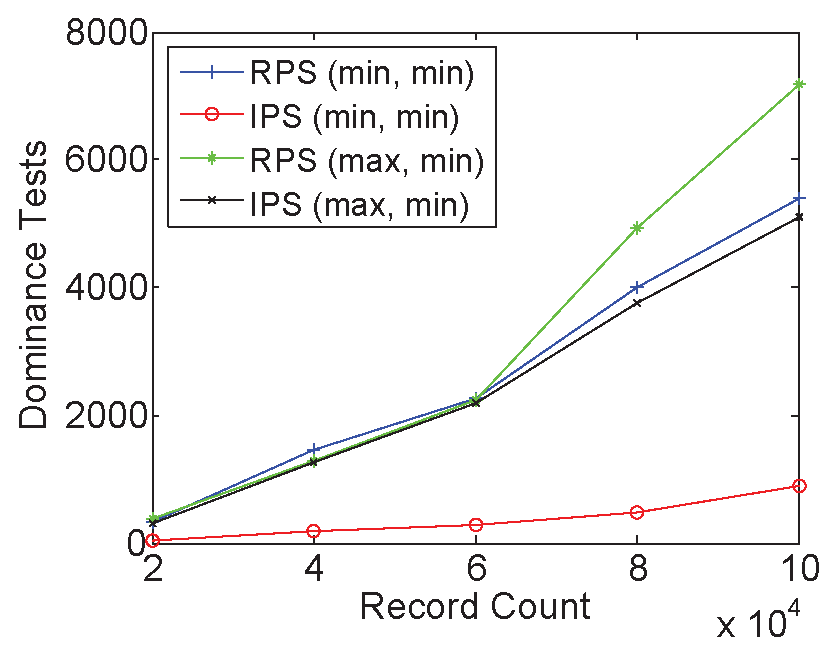
\includegraphics[width=2.5in]{Figures/exp/dt_rc_minmin_maxmin.eps}
    %\end{minipage}
    }
  \subfigure[\small (min, max) and (max, max)]{
    \label{fig:dt_rc_b}
    %\begin{minipage}[h!]{0.5\textwidth}
      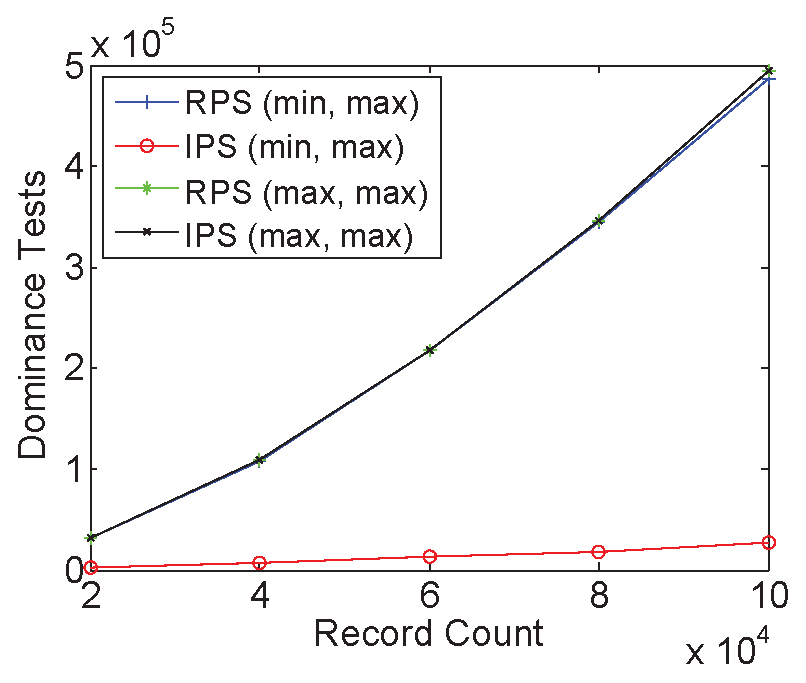
\includegraphics[width=2.5in]{Figures/exp/dt_rc_minmax_maxmax.eps}
    %\end{minipage}
    }
  \caption{\small Dominance Tests vs. Record Count. d = 2, b = 10,
  Data = uniformed}
  \label{fig:dt_rc}
\end{figure}


%%
% Dominance Test vs. Dimensions
%%
\begin{figure}[!h]
  \centering
  \subfigure[\small All Min and All Max. Data = uniformed]{
    \label{fig:dt_dim_a}
    %\begin{minipage}[h!]{0.5\textwidth}
      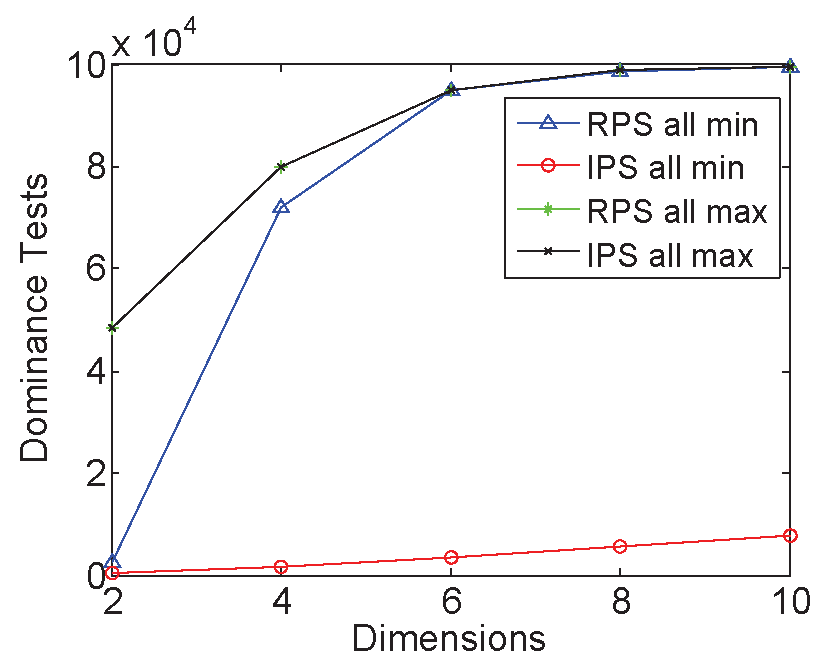
\includegraphics[width=2.5in]{Figures/exp/dt_dim_allmin_allmax.eps}
    %\end{minipage}
    }
  \subfigure[\small Mixed Data Types]{
    \label{fig:dt_dim_b}
    %\begin{minipage}[h!]{0.5\textwidth}
      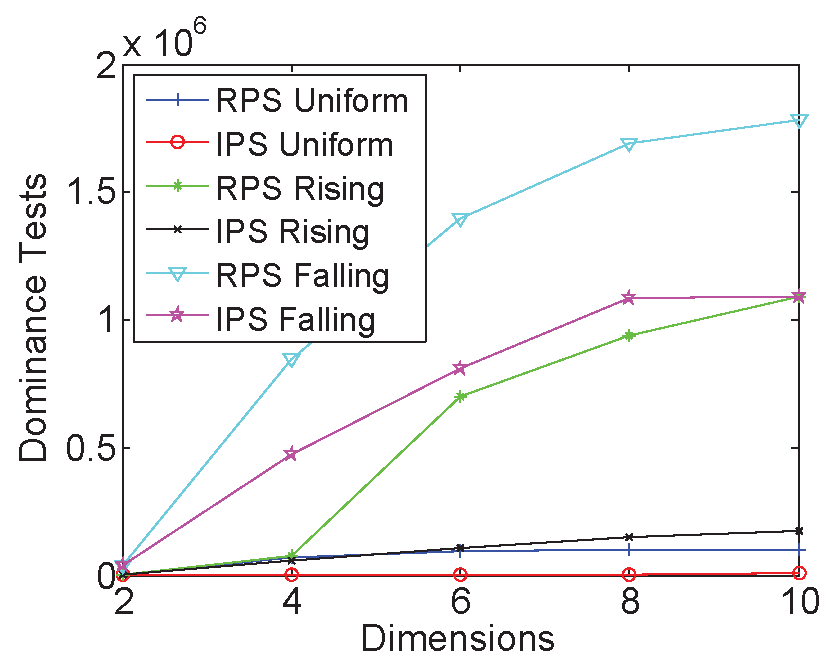
\includegraphics[width=2.5in]{Figures/exp/dt_dim_mixdata_rc10000.eps}
    %\end{minipage}
    }
  \caption{\small Dominance Tests vs. Dimensions. rc = 10000, b = 10}
  \label{fig:dt_dim}
\end{figure}


\subsection{Tuning Time}\label{sec:exp_tuning_time}

As discussed in Section~\ref{sec:wireless_broadcast}, tuning time is the total amount of data the client has to download to fulfill a skyline query. It is measured in bytes. The experiment simulates the creation of the TDI broadcast program by the server. Tuning time is found by simulating a client evaluation of a skyline query from the beginning of the cycle.

Figure~\ref{fig:tt_rec} illustrates tuning time versus increasing record count for all combinations of min and max attribute for 2-dimensional data. In all cases, the IPS performs several factors better than RPS.

Figure~\ref{fig:tt_dim} illustrates the simulation result for tuning time with increasing data dimension. The experiments are run with a record count = 10,000, and a $b$ = 10. Although the number of records stays the same, each additional dimension or data attribute of the data set adds space complexity to the data set. With increasing dimensionality, the cycle length also increases, as well as tuning time.

%%
% Tuning Time vs. Record Count
%%
\begin{figure}[!h]
  \centering
  \subfigure[\small (min, min) and (max, max)]{
    \label{fig:tt_rec_a}
    %\begin{minipage}[h!]{0.5\textwidth}
      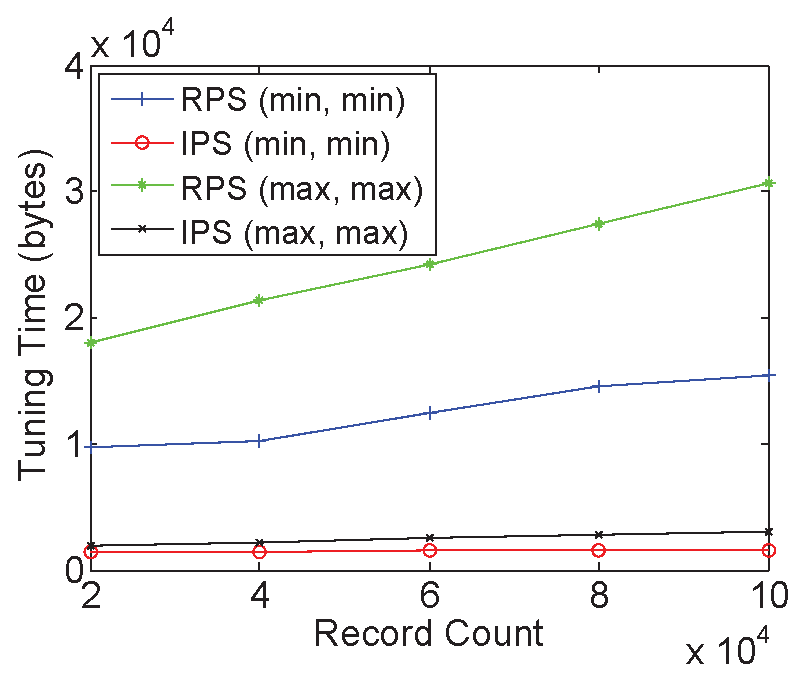
\includegraphics[width=2.5in]{Figures/exp/tt_rc_minmin_maxmax.eps}
    %\end{minipage}
    }
  \subfigure[\small (min, max) and (max, min)]{
    \label{fig:tt_rec_b}
    %\begin{minipage}[h!]{0.5\textwidth}
      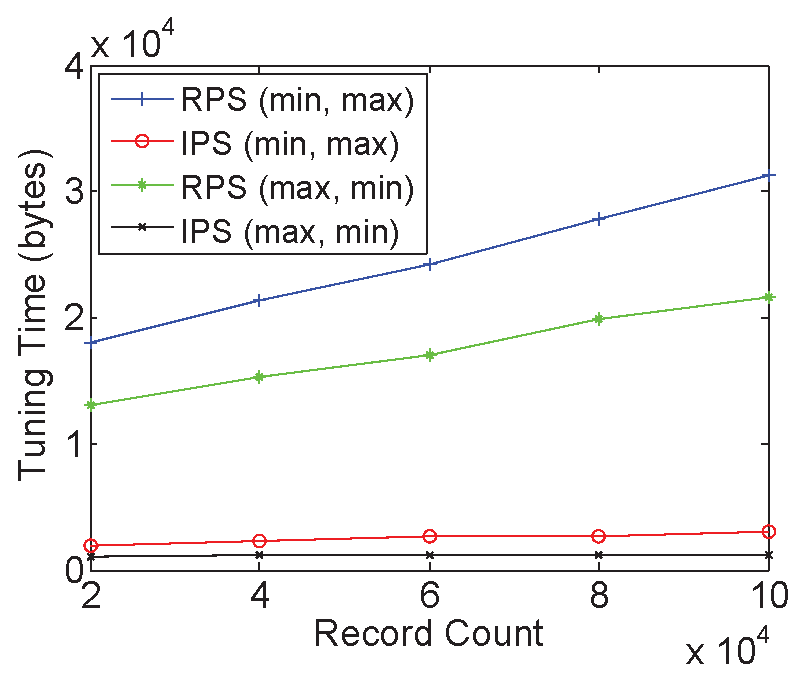
\includegraphics[width=2.5in]{Figures/exp/tt_rc_minmax_maxmin.eps}
    %\end{minipage}
    }
  \caption{\small Tuning Time vs. Record Count. d = 2, b = 10}
  \label{fig:tt_rec}
\end{figure}

%%
% Tuning Time vs. Dimension
%%
\begin{figure}[!h]
  \centering
  \subfigure[\small All Min and All Max]{
    \label{fig:tt_dim_a}
    %\begin{minipage}[h!]{0.5\textwidth}
      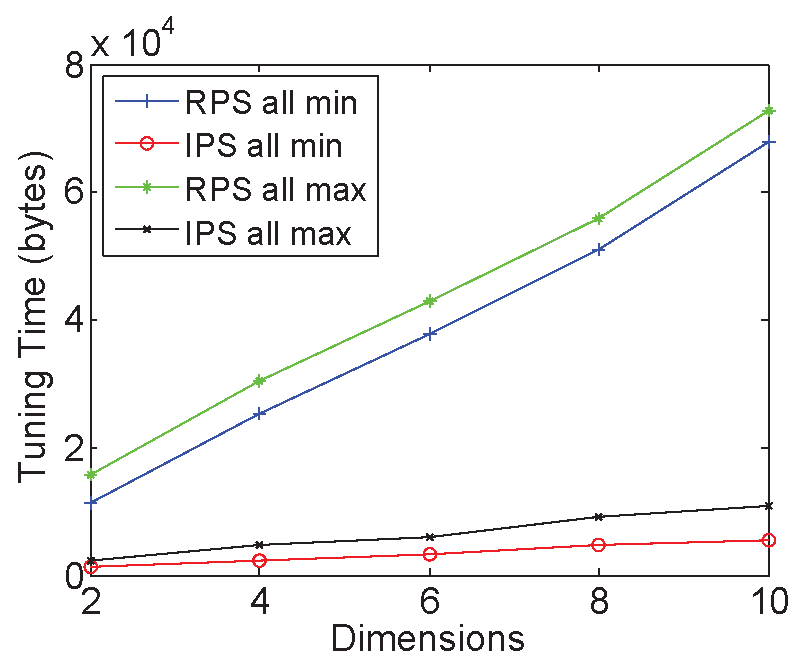
\includegraphics[width=2.5in]{Figures/exp/tt_dim_allmin_allmax_mod.eps}
    %\end{minipage}
    }
  \subfigure[\small Mixed Data Types]{
    \label{fig:tt_dim_b}
    %\begin{minipage}[h!]{0.5\textwidth}
      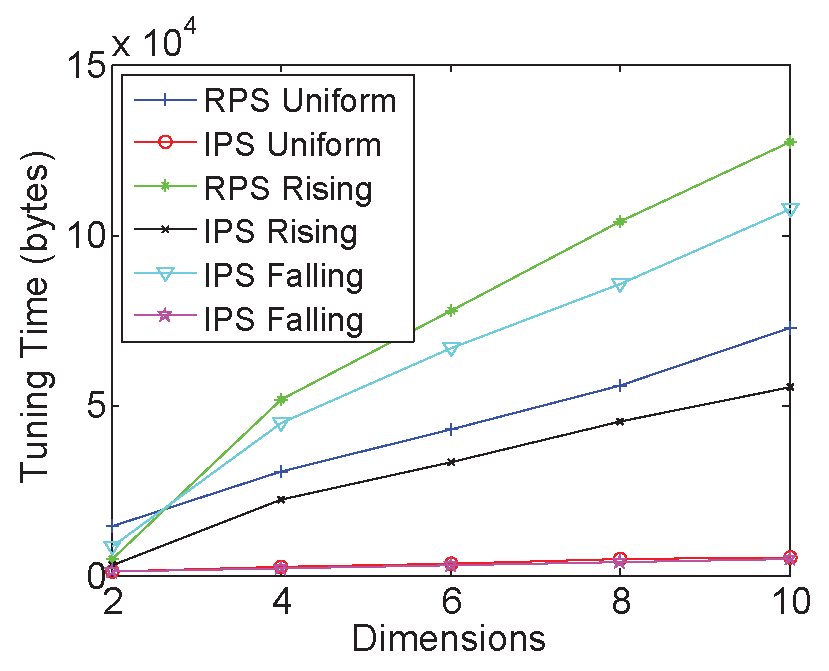
\includegraphics[width=2.5in]{Figures/exp/tt_dim_mixdata_rc10000.eps}
    %\end{minipage}
    }
  \caption{\small Tuning Time vs. Dimensionality. rc = 10000, b = 10}
  \label{fig:tt_dim}
\end{figure}

%%
% Index Percentage
%%
\begin{figure}[!h]
  \centering
  \subfigure[\small IP vs. Record Count]{
    \label{fig:ip_rc}
    %\begin{minipage}[h!]{0.5\textwidth}
      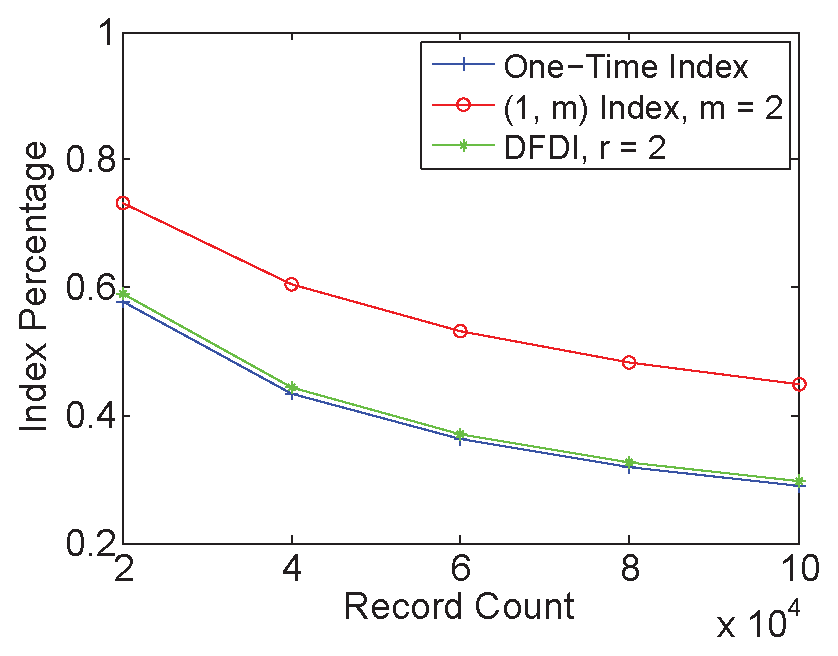
\includegraphics[width=2.5in]{Figures/exp/ip_rc.eps}
    %\end{minipage}
    }
  \subfigure[\small IP vs. Dimensionality]{
    \label{fig:ip_dim}
    %\begin{minipage}[h!]{0.5\textwidth}
      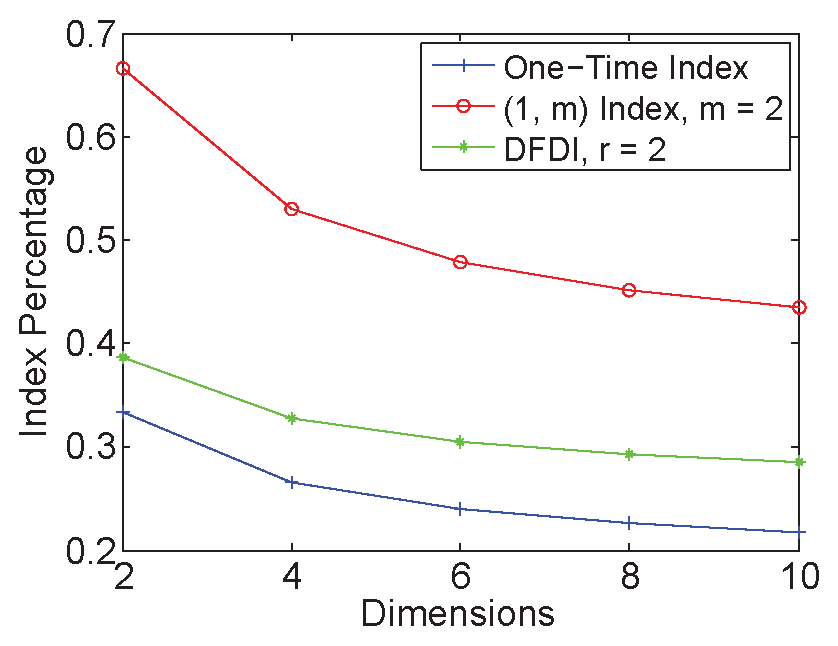
\includegraphics[width=2.5in]{Figures/exp/ip_dim.eps}
    %\end{minipage}
    }
  \caption{\small Index Percentage. b = 10}
  \label{fig:ip}
\end{figure}


\subsection{Index Percentage}

Index percentage measures the efficiency of the TDI broadcast program
allocation technique under increasing record count and increasing data
dimension. Index percentage is defined in
section~\ref{sec:wireless_broadcast}.

Figure~\ref{fig:ip_rc} shows index percentage versus increasing
record count. For the TDI, the simulation is run with a
replication level of 2, which means the root and the first level
below the root are replicated. For the (1, m) index, m = 2,
meaning the complete index is duplicated 2 times in the broadcast
cycle. The figure shows that the overhead of the index is high
when the number of records is low, but the overhead flattens as
the number of records grows. The one-time index is the baseline,
and as expected has the lowest index percentage. Although TDI
replicated the index for 2 levels, its index percentage is only
slightly (16\%) higher than the one-time index. This shows that
TDI is efficient in terms of space overhead, whereas the (1, m)
index has a far worse overhead for only 2 duplications.

Figure~\ref{fig:ip_dim} shows index percentage over increasing
data dimension. The experiment is conducted with 10,000 records
and a branching factor of 10. As the data size grows with the
number of dimensions, the index is only slightly affected by the
growth. The size of the index grows because it needs extra space
to store the information of the extra dimensions, but the tree
height is largely unaffected; thus gives the falling of index
percentage with growing dimension.

%Simulate 3 algorithms:
%\begin{enumerate}
%\item R-Tree one-time index \item R-Tree TDI \item Grid R-Tree
%TDI
%\end{enumerate}

%Measurements:
%\begin{enumerate}
%\item Index percentage (with variable branching factor) \item
%Tuning time (with variable branching factor) \item Dominance tests
%(with variable branching factor)
%\end{enumerate}


%\section{Conclusion}\label{bsky-conc}
%In this work, we presented a technique for efficient skyline computation in broadcast environment. To make the broadcast program self-descriptive, we used an R-Tree to index broadcast data records. We then introduced Tree-Based Distributed Index (TDI) program allocation, in which the index and data records are serialized and pushed to the broadcast channel.

In addition, we presented two algorithms (RPS and IPS) for evaluating skyline results from TDI broadcast program. Ours is only work we know that is able to evaluate skyline for data record with arbitrary dimensions and arbitrary skyline preferences.

Our simulation results with synthetic data show that our program allocation technique create program with low index overhead. In addition, our skyline algorithms performs well with variety of data-sets.

%In this paper, we presented a broadcast data stream allocation technique (TDI) that utilizes the R-tree and performs a depth-first traversal of the index to create a distributed index. The goals of TDI are to facilitate query processing from broadcast data, to reduce the index overhead (IP) and to improve the initial index probe. TDI is able to achieve all these with reasonable efficiency. TDI is a flexible R-tree based index and supports skyline queries as well as other data query types. The allocation distributes $b^h$ number of index segments among the broadcast program to reduce the initial index, and at the same time keeps the index overhead low. The simulation results for index percentage show that TDI performs very well with two levels of replication and follow the efficiency of one-time index with only a $16\%$ increase in index overhead.

%The simulation results show that the approach also performs well with data of higher dimensions. The index overhead decreases as the number of records remain constant and the number of data dimensions increase. This is due to the fact that the growth of dimensionality does not make the index tree grow ``taller" and does not incur the cost of new nodes when the index grows. The height of an index tree does increase as the number of records increase, but as seen in Figure~\ref{fig:ip_rc}, the growth of the index is not as fast as the growth of the amount of data; therefore, the index overhead decreases as records increase.

%In addition, we introduced point-based and index-based pruning skyline algorithms. The experiments show that both algorithms are capable of evaluating skyline queries of combined $min$ and $max$ attributes with reasonable tuning time and dominance tests. The index-based skyline has always performed better than the point-based skyline, in some cases by several factors. The performance of the algorithms is also affected by the data arrangement and R-tree implementation. From our simulation, we find that R-trees that index records with lower attributes first perform better for $min$ skyline queries, and vice versa.

%\section*{Acknowledgements}
%
This research has been funded in part by the National Science
Foundation (NSF) Grants CNS-0831502 (CT) and CNS-0855251 (CRI).

%Any opinions, findings, and conclusions or recommendations
%expressed in this material are those of the author(s) and do not
%necessarily reflect the views of the National Science Foundation.


%\small {\section*{Acknowledgments}


%\bibliographystyle{abbrv}
%\bibliography{bibliography}

%\end{document}
